\documentclass[11pt, english]{article}\usepackage[]{graphicx}\usepackage[]{color}
%% maxwidth is the original width if it is less than linewidth
%% otherwise use linewidth (to make sure the graphics do not exceed the margin)
\makeatletter
\def\maxwidth{ %
  \ifdim\Gin@nat@width>\linewidth
    \linewidth
  \else
    \Gin@nat@width
  \fi
}
\makeatother

\definecolor{fgcolor}{rgb}{0.345, 0.345, 0.345}
\newcommand{\hlnum}[1]{\textcolor[rgb]{0.686,0.059,0.569}{#1}}%
\newcommand{\hlstr}[1]{\textcolor[rgb]{0.192,0.494,0.8}{#1}}%
\newcommand{\hlcom}[1]{\textcolor[rgb]{0.678,0.584,0.686}{\textit{#1}}}%
\newcommand{\hlopt}[1]{\textcolor[rgb]{0,0,0}{#1}}%
\newcommand{\hlstd}[1]{\textcolor[rgb]{0.345,0.345,0.345}{#1}}%
\newcommand{\hlkwa}[1]{\textcolor[rgb]{0.161,0.373,0.58}{\textbf{#1}}}%
\newcommand{\hlkwb}[1]{\textcolor[rgb]{0.69,0.353,0.396}{#1}}%
\newcommand{\hlkwc}[1]{\textcolor[rgb]{0.333,0.667,0.333}{#1}}%
\newcommand{\hlkwd}[1]{\textcolor[rgb]{0.737,0.353,0.396}{\textbf{#1}}}%
\let\hlipl\hlkwb

\usepackage{framed}
\makeatletter
\newenvironment{kframe}{%
 \def\at@end@of@kframe{}%
 \ifinner\ifhmode%
  \def\at@end@of@kframe{\end{minipage}}%
  \begin{minipage}{\columnwidth}%
 \fi\fi%
 \def\FrameCommand##1{\hskip\@totalleftmargin \hskip-\fboxsep
 \colorbox{shadecolor}{##1}\hskip-\fboxsep
     % There is no \\@totalrightmargin, so:
     \hskip-\linewidth \hskip-\@totalleftmargin \hskip\columnwidth}%
 \MakeFramed {\advance\hsize-\width
   \@totalleftmargin\z@ \linewidth\hsize
   \@setminipage}}%
 {\par\unskip\endMakeFramed%
 \at@end@of@kframe}
\makeatother

\definecolor{shadecolor}{rgb}{.97, .97, .97}
\definecolor{messagecolor}{rgb}{0, 0, 0}
\definecolor{warningcolor}{rgb}{1, 0, 1}
\definecolor{errorcolor}{rgb}{1, 0, 0}
\newenvironment{knitrout}{}{} % an empty environment to be redefined in TeX

\usepackage{alltt}
\usepackage{amsmath,amssymb,latexsym}

%\usepackage{palatino}
%\usepackage{arev}
\usepackage{fourier}
%\usepackage{antpolt}

\usepackage{graphicx}
\usepackage{tikz-qtree}
\usepackage{amscd}
\usepackage{bbm}
\usepackage{caption}
\usepackage[utf8]{inputenc}
\usepackage[T1]{fontenc}
\usepackage{babel}
\usepackage{rotating,amssymb,amsmath,amsfonts,delarray}
\usepackage{geometry}
\usepackage{placeins}
\usepackage{caption}
\usepackage{float}
\usepackage{amsthm}
\newtheorem*{remark}{Remark}
\geometry{hmargin=80pt, vmargin=70pt}
\usepackage{amsfonts}
\usepackage{xcolor}
\usepackage{hyperref}
\usepackage{enumerate}
\usepackage{enumitem}
\usepackage{tikz}
\usepackage{cancel}
\usepackage{scalerel,stackengine}

\usepackage{forest}

\colorlet{mygreen}{green!75!black}
\colorlet{col1in}{red!30}
\colorlet{col1out}{red!40}
\colorlet{col2in}{mygreen!40}
\colorlet{col2out}{mygreen!50}
\colorlet{col3in}{blue!30}
\colorlet{col3out}{blue!40}
\colorlet{col4in}{mygreen!20}
\colorlet{col4out}{mygreen!30}
\colorlet{col5in}{blue!10}
\colorlet{col5out}{blue!20}
\colorlet{col6in}{blue!20}
\colorlet{col6out}{blue!30}
\colorlet{col7out}{orange}
\colorlet{col7in}{orange!50}
\colorlet{col8out}{orange!40}
\colorlet{col8in}{orange!20}
\colorlet{linecol}{blue!60}

\hypersetup{
  colorlinks=true,
  citecolor=blue,
  linkcolor=blue,
  filecolor=magenta,
  urlcolor=cyan,
}

\newtheorem{rem}{Remark}
\newtheorem{deff}{Definition}
\newtheorem{lem}{Lemma}
\newtheorem{ex}{Example}
\newtheorem{theorem}{Theorem}
\newtheorem{algo}{Algorithm}

\setlength{\parindent}{0cm}

\setlength\parindent{0pt}

\title{The \texttt{nCopula} package}
\author{David Beauchemin \\ Simon-Pierre Gadoury}
\date{\today}
\IfFileExists{upquote.sty}{\usepackage{upquote}}{}
\begin{document}

\maketitle

\begin{abstract}
The \emph{nCopula} package aims to simplify the construction process and usage of hiearchical Archimedean copulas through compound distributions in \texttt{R}. Is is possible to build structures with clear representations, obtain expressions for Archimedean copulas, wether they are hiearchical or not, as well as other important functions (i.e. Laplace Stieltjes Transform, pgf, etc.), given a certain path and structure. Furthermore, the generation of random vectors is possible from any given structure.
\end{abstract}

\section{Introduction}

Copulas are now well known tools used for dependence modeling purposes in
many research topics. A $d$-dimensional copula is a $d$-variate probability
distribution function for which the marginals are uniformly distributed on $%
(0,1)$, with $d\geq 2$. One important class of copulas is the Archimedean
copula family, popular for its simple construction procedure and
multivariate generalization. A $d$-dimensional copula $C$ is said to be an \emph{Archimedean
copula} if
\begin{equation}
C(u_{1},\ldots ,u_{d})=\psi \left( \psi ^{-1}(u_{1})+\ldots +\psi
^{-1}(u_{d})\right) ,\,\,\text{for}\,\,(u_{1},\ldots ,u_{d})\in \lbrack
0,1]^{d}.  \label{eq1}
\end{equation}%
The continuous and strictly decreasing function $\psi $ is called the
generator of the copula, where $\psi :[0,\infty )\rightarrow \lbrack 0,1]$, $%
\psi (0)=1$ and $\displaystyle\lim_{t\rightarrow \infty }\psi (t)=0$. In
the same manner, $\psi ^{-1}:[0,1]\rightarrow \lbrack 0,\infty )$, for which
  $\psi ^{-1}(0)=\inf
\{t:\psi (t)=0\}$, where $\psi ^{-1}$ is the inverse of the generator $\psi $%
. The set of all such functions is denoted by $\Psi_\infty$. In fact, from Kimberling's and Bernstein's theorems, see e.g. \cite%
{kimberling}, \cite{feller}, and \cite{hofert}, representation (\ref{eq1})
leads to a proper copula for all $d\geq 2$ if and only if $\psi $ is the
Laplace-Stieltjes Transform (LST) of a strictly positive random variable (rv) $\Theta $ with cumulative distribution function (cdf) $F_{\Theta}$, where the LST of the rv $\Theta $ is given by
\begin{equation}
  \mathcal{L}_{\Theta}(t) = \int_{0}^{\infty} \mathrm{e}^{-t \, x} \, \mathrm{d} F_{\Theta}(x)=E\left[\mathrm{e}^{-t{\Theta}}\right].
\end{equation}

The use of multivariate Archimedean copulas in high dimension can be
restrictive due to their exchangeability property. One can resort to
another interesting class of copulas, namely vine copulas (see e.g. \cite{bedford2002} and \cite{joe1997}). They are pair copula constructions
allowing a cascade decomposition of a multivariate distribution into the
product of bivariate copulas. Vine copulas force the use of $\frac{d(d-1)}{2%
}$ bivariate copulas which requires a high number of parameters when $d$,
the dimension of the copula, increases. \\


Hierarchical Archimedean copulas provide an interesting alternative to allow asymmetries.
The first approach to construct hierarchical Archimedean copulas was proposed by \cite{joe1997} who introduced the so-called nested Archimedean copulas in three and four dimensions. They
are obtained by nesting into each other Archimedean copulas.
They are able to capture different dependence relations between and within different
groups of risks with a relatively small number of parameters (see e.g. \cite{gorecki2016}). They were further studied by e.g. \cite{mcsample08}, \cite{hofert12eff}, and \cite{hofert11eff}, in a general setting.  For an Archimedean hierarchical structure to be a
proper copula, a given nesting condition must be verified. For example, a
3-dimensional fully nested Archimedean copula can be written as
\begin{equation*}
C(u_{1},u_{2},u_{3})=C(u_{1},C(u_{2},u_{3}))=\psi _{0}\Big(\psi
_{0}^{-1}(u_{1})+\psi _{0}^{-1}\circ \psi _{1}\big(\psi
_{1}^{-1}(u_{2})+\psi _{1}^{-1}(u_{3})\big)\Big).
\end{equation*}

For the hierarchical structure to be a proper copula, $\psi _{0}^{-1}\circ
\psi _{1}$ must have completely monotone derivatives, where $\psi _{0}$ and $%
\psi _{1}$ are generators of the parent and the child copulas respectively.
If generators $\psi _{0}$ and $\psi _{1}$ belong to the same family, the
verification of this sufficient nesting condition can be done without much
problem, see \cite{hofert} for restrictions on the parameters. \\

The \emph{copula} package implements serveral very effective functions to construct and use nested Archimedean copulas (see \cite{hofert2011nested}).

\section{Hierarchical Archimedean copulas through compounding}

(...) \\

\begin{knitrout}
\definecolor{shadecolor}{rgb}{0.969, 0.969, 0.969}\color{fgcolor}\begin{kframe}


{\ttfamily\noindent\itshape\color{messagecolor}{\#\# Loading required package: copula}}

{\ttfamily\noindent\color{warningcolor}{\#\# Warning: package 'copula' was built under R version 3.3.2}}\end{kframe}
\end{knitrout}

Let us consider a two level tree $\lambda = \{(0,1,1), (0,1,2), (0,2)\}$, as illustrated in Figure~\ref{fig:ex1}.

\begin{figure}[!h]
\[
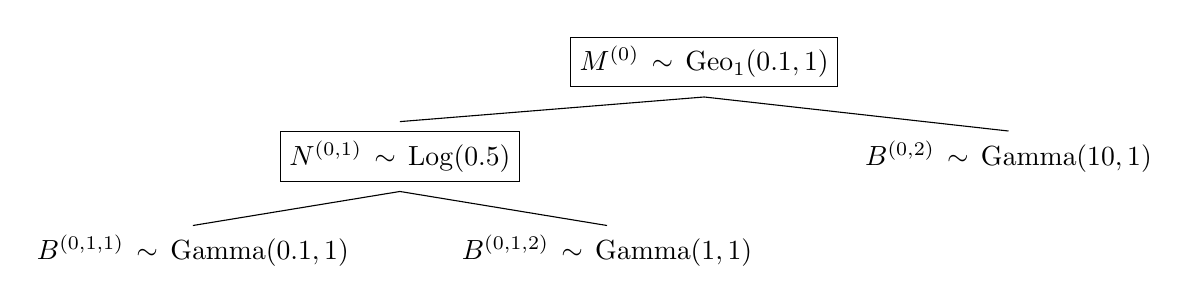
\begin{tikzpicture}[scale=1, level distance=12mm, sibling distance=12mm]
\Tree [.\fbox{$M^{(0)}\,\sim\,\mathrm{Geo}_1(0.1,1)$}
        [.\fbox{$N^{(0,1)}\,\sim\,\mathrm{Log}(0.5)$} $B^{(0,1,1)}\,\sim\,\mathrm{Gamma}(0.1,1)$ $B^{(0,1,2)}\,\sim\,\mathrm{Gamma}(1,1)$ ]
      [.$B^{(0,2)}\,\sim\,\mathrm{Gamma}(10,1)$ ] ]
\end{tikzpicture}
\]
\caption{Two level structure}\label{fig:ex1}
\end{figure}

\begin{knitrout}\scriptsize
\definecolor{shadecolor}{rgb}{0.969, 0.969, 0.969}\color{fgcolor}\begin{kframe}
\begin{alltt}
\hlstd{str} \hlkwb{<-} \hlkwd{GEO}\hlstd{(}\hlnum{0.1}\hlstd{,} \hlkwa{NULL}\hlstd{,} \hlkwd{list}\hlstd{(}\hlkwd{LOG}\hlstd{(}\hlnum{0.5}\hlstd{,} \hlkwa{NULL}\hlstd{,} \hlkwd{list}\hlstd{(}\hlkwd{GAMMA}\hlstd{(}\hlnum{0.1}\hlstd{,} \hlnum{1}\hlopt{:}\hlnum{2}\hlstd{,} \hlkwa{NULL}\hlstd{),}
                                               \hlkwd{GAMMA}\hlstd{(}\hlnum{1}\hlstd{,} \hlnum{3}\hlopt{:}\hlnum{4}\hlstd{,} \hlkwa{NULL}\hlstd{))),}
                           \hlkwd{GAMMA}\hlstd{(}\hlnum{10}\hlstd{,} \hlnum{5}\hlopt{:}\hlnum{6}\hlstd{,} \hlkwa{NULL}\hlstd{)))}

\hlstd{str}
\end{alltt}
\begin{verbatim}
##  Shifted geometric distribution: 2-dimensional 'Mother' function with parameter 0.1
##  composed of (2) children: 
## 
##     1) Logarithmic distribution: 2-dimensional 'Mother' function with parameter 0.5
##        composed of (2) children: 
## 
##        1) Gamma distribution: 2-dimensional 'Child' function with parameter 0.1 
##           composed of (u1, u2) 
## 
##        2) Gamma distribution: 2-dimensional 'Child' function with parameter 1 
##           composed of (u3, u4) 
## 
##     2) Gamma distribution: 2-dimensional 'Child' function with parameter 10 
##        composed of (u5, u6)
\end{verbatim}
\end{kframe}
\end{knitrout}


\newpage

\bibliographystyle{apalike}
\bibliography{BibRRT}

\end{document}
